\documentclass[10pt]{beamer}

\usetheme{Copenhagen}
\usepackage[italian]{babel}
\usepackage[utf8x]{inputenc}
\usepackage {eurosym}
\setbeamercovered{transparent}

%
% The following info should normally be given in you main file:
%
\setbeamertemplate{footline}{
\hfill\insertframenumber/\inserttotalframenumber
}
\pgfdeclareimage[height=5mm]{logo}{logo.png}
\logo{\pgfuseimage{logo}}

\title{Revisione dei requisiti}
\titlegraphic{\pgfuseimage{logo}}
\author{Grosselle Alessandro, Barbiero Mattia}
\date{12 Dicembre 2008}


\begin{document}
\transduration{1}

\frame{
	\transsplitverticalin
	\titlepage }


\section*{Sommario}

\subsection{1a Parte: Introduzione}

\frame{
  \transsplitverticalin
  \nameslide{outline}
  \frametitle{Introduzione}
  \tableofcontents[pausesections,part=1]
}

\subsection{2a Parte: Requisiti}

\frame{
  \transsplitverticalin
  \nameslide{outline}
  \frametitle{Descrizione requisiti}
  \tableofcontents[pausesections,part=2]
}

\subsection{3a Parte: Use case del sistema}

\frame{
  \transsplitverticalin
  \nameslide{outline}
  \frametitle{Use case del sistema}
  \tableofcontents[pausesections,part=3]
}

\part{Introduzione}

\frame{
	\transsplitverticalin
	\partpage }

\section{Introduzione}
\subsection{Capitolato d'appalto}
\frame{
	\frametitle{Introduzione}
  \framesubtitle{Capitolato d'appalto: ''SIGEOL''}
  \emph{Azienda Committente}: Prof. Rossi, rappresentata dai docenti proff. Vardanega e Conte.
  
  
  Il presente capitolato ha per oggetto l'affidamento della fornitura di un sistema software per la gestione dell'orario di lezione a uso del presidente del CCS di Informatica.
  
  \transsplitverticalin
	 }
\subsection{Scopo del prodotto}
\frame{
	\frametitle{Introduzione}
  \framesubtitle{Scopo del prodotto}
  Il progetto sotto analisi, denominato \textit{SIGEOL}, si prefigge di automatizzare la generazione, la gestione, l'ottimizzazione e la consultazione degli orari di lezione. Il committente richiede l'applicazione del sistema al solo corso di laurea in Informatica, ma, constatato che la complessità non aumenta notevolmente, il team QuiXoft prevede lo sviluppo e la messa in opera dell'applicazione per tutti i corsi di laurea dell' Università degli studi di Padova.
  \transsplitverticalin
	 }
\subsection{Contesto d'uso del prodotto}
\frame{
	\frametitle{Introduzione}
  \framesubtitle{Contesto d'uso del prodotto}
  \begin{itemize}

  \item Processi produttivi e modalità d'uso: Il funzionamento del sistema \textit{SIGEOL}, a processo produttivo concluso, sarà in grado di guidare ogni singolo utilizzatore allo svolgimento delle proprie azioni. In altre parole sarà disponibile un servizio che offrirà, dopo un'opportuna autenticazione, un insieme di strumenti che permetteranno l'inserimento guidato dei dati che serviranno al fine ultimo di generare un orario per le lezioni.
  \item Piattaforma d'esecuzione ed interfacciamento con l'ambiente di installazione e uso: Il prodotto sarà realizzato tramite un'applicazione web supportata da un database e dovrà essere accessibile da un qualsiasi tipo di browser. 
  \end{itemize}
  \transsplitverticalin
	 }
\subsection{Caratteristiche degli utenti}
\frame{
	\frametitle{Introduzione}
  \framesubtitle{Caratteristiche degli utenti}
  Si prevedono cinque tipologie di utenti che usufruiranno del sistema:
\begin{itemize}
 \item Segreteria generale: si occupa dell'invito delle varie \textit{segreterie didattiche}, nonchè della preparazione della struttura delle varie facoltà
 \item Segreteria didattica: ha, tra gli altri, il compito di invitare i \textit{presidenti del CCS} dei vari corsi di laurea e di inserire i corsi della facoltà di sua competenza.
 \item Presidente del CCS: provvede, invece, all'invito dei vari \textit{docenti}. 
 \item Docente: dovranno compilare i propri dati ed accettare il consenso al loro trattamento. 
 \item Utente non autenticato: sarà in grado di consultare le informazioni che verranno rese disponibili dal sistema, quali schemi d'orario, informazioni su docenti, aule, corsi di laurea e corsi.
\end{itemize}
  \transsplitverticalin
	 }

\subsection{Stime sul prodotto}
\frame{
	 \frametitle{Introduzione}
   \framesubtitle{Stime sul prodotto}
   \begin{itemize}
   \item Costo del Prodotto: Il costo del prodotto è stato stimato intorno a 13065\euro.
   \item Data di termine: Si prevede di terminare il progetto entro il 23 Marzo 2009.
   \item Ore per risora: Ogni componente del gruppo avrà un carico di lavoro compreso tra le 103.5 e le 105.5 ore 
   \transsplitverticalin
	 \end{itemize}
	 }

\part{Descrizione dei requisiti}
\frame{
	\transsplitverticalin
	\partpage }
\section{Descrizione dei requisiti}
\subsection{Requisiti Funzionali}
\subsubsection{Requisiti Funzionali per la segreteria generale}
\frame{
  \frametitle{Requisiti Funzionali}
  \framesubtitle{Requisiti Funzionali per la segreteria generale}
  \begin{itemize}
   \item Possibilità di autenticazione
   \item Possibilità di inserimento delle facoltà
   \item Possibilità di invitare le singole facoltà ad inserire i dati
   \item Possibilità di consultare lo schema d'orario di ogni corso di laurea
  \end{itemize}
  \transsplitverticalin
  }
\subsubsection{Requisiti funzionali per la segreteria didattica}
\frame{
 \frametitle{Requisiti Funzionali}
 \framesubtitle{Requisiti Funzionali per la segreteria didattica}
 \begin{itemize}
 \item Possibilità di autenticazione
 \item Possibilità di inserimento e modifica per ogni corso, all'interno della propria facoltà, del nome, dei relativi CFU,   dell'anno di appartenenza, del periodo, dello stato, del numero di ore in aula e in laboratorio (se previsto), del docente di  riferimento che lo tiene, di eventuali assistenti e della stima del numero di studenti che lo seguiranno
 \item Possibilità di inserimento e modifica per ogni aula disponibile, all'interno della propria facoltà, del nome, della capienza, delle ore e dei periodi di non disponibilità
 \item Possibilità di inserimento e modifica dell'anno accademico
 \end{itemize}
 \transsplitverticalin
 }
\frame{
 \frametitle{Requisiti Funzionali}
 \framesubtitle{Requisiti Funzionali per la segreteria didattica}

 \begin{itemize}
   \item Possibilità di impostare vincoli e preferenze per ogni corso di laurea
   \item Possibilità di modifica dei dati dei docenti preventivamente inseriti dal Presidente del CCS
   \item Possibilità di invitare via e-mail i presidenti del CCS di ogni corso di laurea ad inserire i dati
   \item Possibilità di ripristinare i dati relativi ai corsi di laurea da un backup scelto
 \end{itemize}  
 \transsplitverticalin
 }
\subsubsection{Requisiti funzionali per il Presidente del CCS}
\frame{
 \frametitle{Requisiti Funzionali}
 \framesubtitle{Requisiti Funzionali per il Presidente del CCS}
 \begin{itemize}
\item Possibilità autenticazione
\item Possibilità di inserimento e modifica per ogni corso, all'interno del proprio corso di laurea, del nome, dei relativi CFU, dell'anno di appartenenza, del periodo, dello stato, del numero di ore in aula e in laboratorio (se previsto), del docente di riferimento che lo tiene, di eventuali assistenti e della stima del numero di studenti che lo seguiranno
\item Possibilità di inserimento e modifica per ogni aula disponibile, all'interno del proprio corso di laurea, del nome, della capienza, delle ore e dei periodi di non disponibilità
\item Possibilità di inserimento e modifica, all'interno del proprio corso di laurea, dei dati dei docenti
\end{itemize}
}
\frame{
 \frametitle{Requisiti Funzionali}
 \framesubtitle{Requisiti Funzionali per il Presidente del CCS}
 \begin{itemize}
  \item Possibilità di inserimento e modifica dell'anno accademico
  \item Possibilità di impostare vincoli e preferenze per ogni corso
  \item Possibilità di generazione dello schema d'orario in formato pdf e html
  \item Possibilità di scegliere vincoli da rilassare proposti dal sistema in caso di soluzione inesistente
  \item Possibilità di consultare lo schema d'orario
  \item Possibilità di inserimento e modifica di indirizzi diversi appartenenti allo stesso corso di laurea
  \item Possibilità di ripristinare i dati relativi ai corsi da un backup scelto
  \item Possibilità di notificare i docenti nel caso di vincoli e preferenze non soddisfatti.
\end{itemize}
  }

\subsubsection{Requisiti funzionali per i docenti}
\frame{
 \frametitle{Requisiti Funzionali}
 \framesubtitle{Requisiti Funzionali per i docenti}
 \begin{itemize}
\item Possibilità di inserimento e modifica dei propri giorni e ore di indisponibilità, con relativa motivazione
\item Possibilità di inserimento e modifica delle proprie preferenze su orari e giorni di lezione, con relativa motivazione
\item Possibilità di modifica dei propri dati personali
\end{itemize}
}
\subsubsection{Requisiti funzionali(desiderabili) per l'utente non autenticato}
\frame{
 \frametitle{Requisiti Funzionali}
 \framesubtitle{Requisiti Funzionali(desiderabili) per l'utente non autenticato}
 \begin{itemize}
\item Possibilità di consultare lo schema d'orario
\item Possibilità di consultare le informazioni relative a docenti, aule, corsi di laurea e corsi
\end{itemize}
}
\subsection{Requisiti di qualità}
\frame{
  \frametitle{Requisiti di qualità}
  \begin{itemize}
   \item Accessibilità del sistema
   \item Garanzie sull'integrità dei dati
   \item Gestione in sicurezza degli account
   \item Manutenibilità del sistema
   \item Interfaccia utente semplice e intuitiva
   \item Presenza di manuali d'uso, di installazione, configurazione e manutenzione del sistema
   \item Il prodotto dovrà essere consegnato assieme ad un ambiente di prova per verificarne il corretto funzionamento
  \end{itemize}
  \transsplitverticalin
	 }
\subsection{Requisiti d'interfacciamento e d'ambiente}
\frame{
	\frametitle{Requisiti d'interfacciamento e d'ambiente}
 	\begin{itemize}
  \item Le informazioni andranno memorizzate in modo permanente in un \underline{database}
  \end{itemize}
 \transsplitverticalin
	 }
\part{Schemi esplicativi e casi d'uso del prodotto}
\frame{
	\transsplitverticalin
	\partpage }
\subsection{Schema generale}
\frame{
	\frametitle{Schema generale}
	\begin{center}
 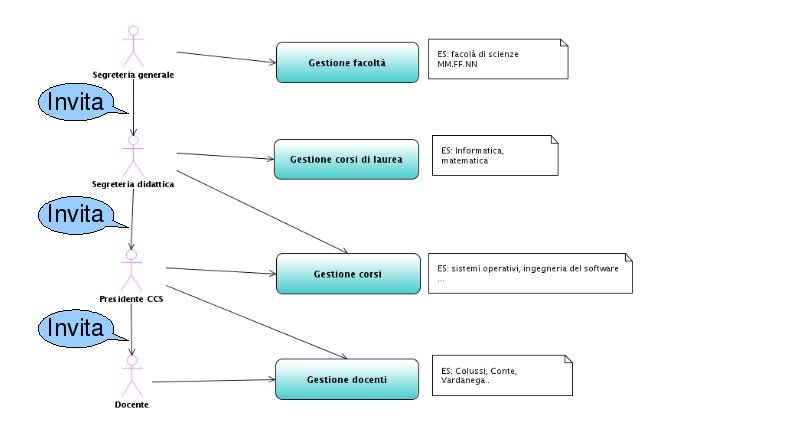
\includegraphics[scale=0.3]{PresentazioneGenerali.jpg}
 % PresentazioneGenerali.jpg: 794x1123 pixel, 72dpi, 28.01x39.62 cm, bb=0 0 794 1123
\end{center}

	\transsplitverticalin
	 }
\subsection{Gestione delle notifiche}
\frame{
	\frametitle{Gestione delle notifiche}

\begin{center}
 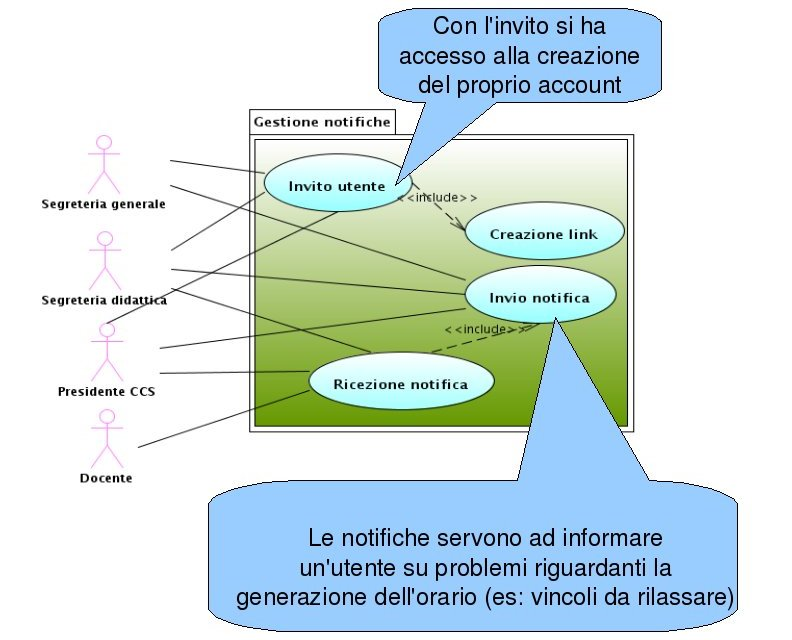
\includegraphics[scale=0.3]{PresentazioneNotifiche.jpg}
 % PresentazioneNotifiche.jpg: 794x1123 pixel, 72dpi, 28.01x39.62 cm, bb=0 0 794 1123
\end{center}
	\transsplitverticalin
	 }
\subsection{Gestione dei corsi}
\frame{
	\frametitle{Gestione dei corsi}

\begin{center}
 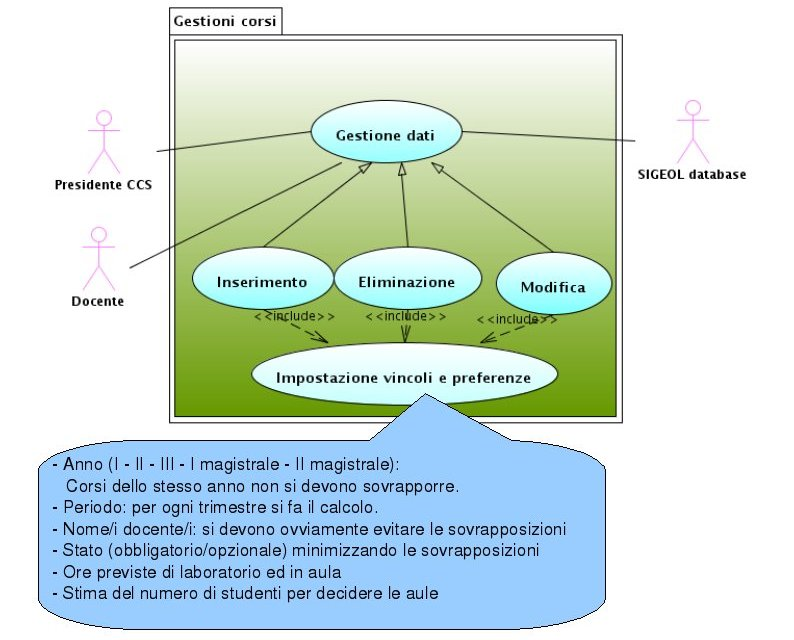
\includegraphics[scale=0.3]{PresentazioneCorsi.jpg}
 % PresentazioneCorsi.jpg: 794x1123 pixel, 72dpi, 28.01x39.62 cm, bb=0 0 794 1123
\end{center}

	\transsplitverticalin
	 }
\subsection{Gestione dei docenti}
\frame{
	\frametitle{Gestione dei docenti}
\begin{center}
 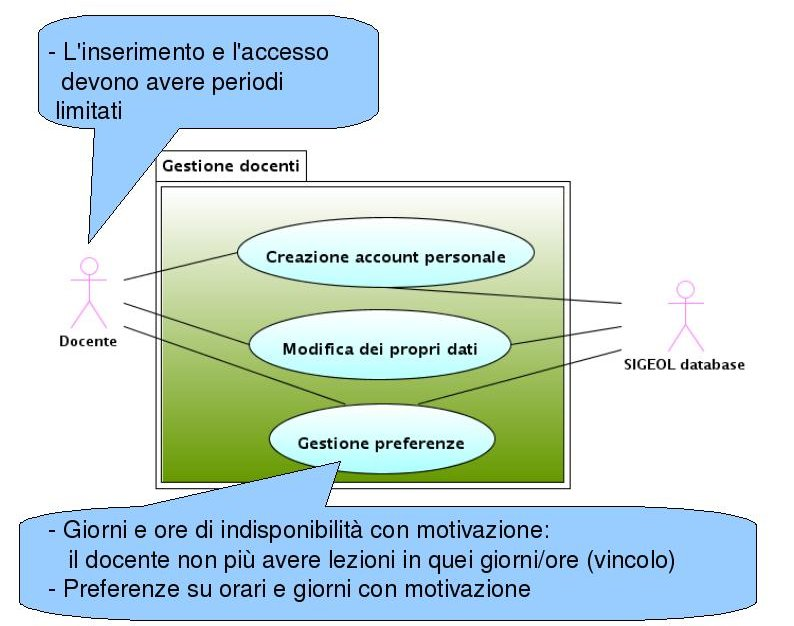
\includegraphics[scale=0.3]{PresentazioneDocenti.jpg}
 % PresentazioneDocenti.jpg: 794x1123 pixel, 72dpi, 28.01x39.62 cm, bb=0 0 794 1123
\end{center}

	\transsplitverticalin
	 }
\subsection{Gestione delle aule}
\frame{
	\frametitle{Gestione delle aule}

\begin{center}
 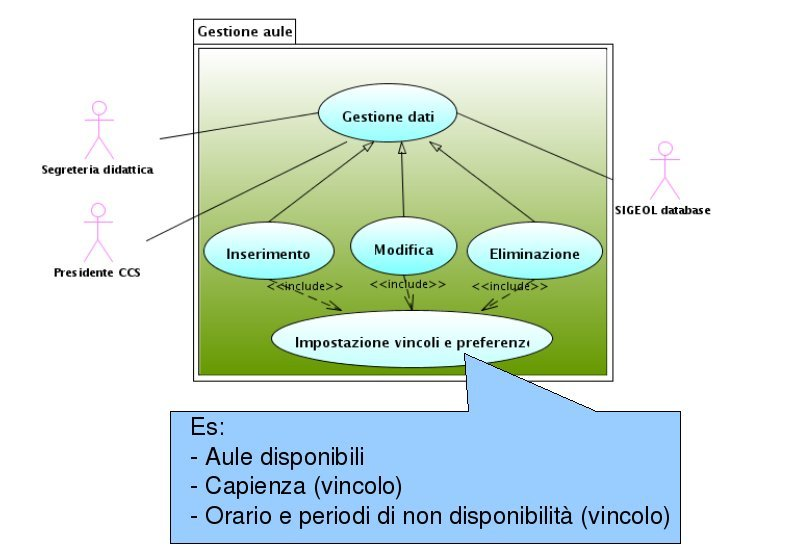
\includegraphics[scale=0.3]{PresentazioneAule.jpg}
 % PresentazioneAule.jpg: 794x1123 pixel, 72dpi, 28.01x39.62 cm, bb=0 0 794 1123
\end{center}

	\transsplitverticalin
	 }
\subsection{Generazione dello schema d'orario}
\frame{
	\frametitle{Generazione dello schema d'orario}

\begin{center}
 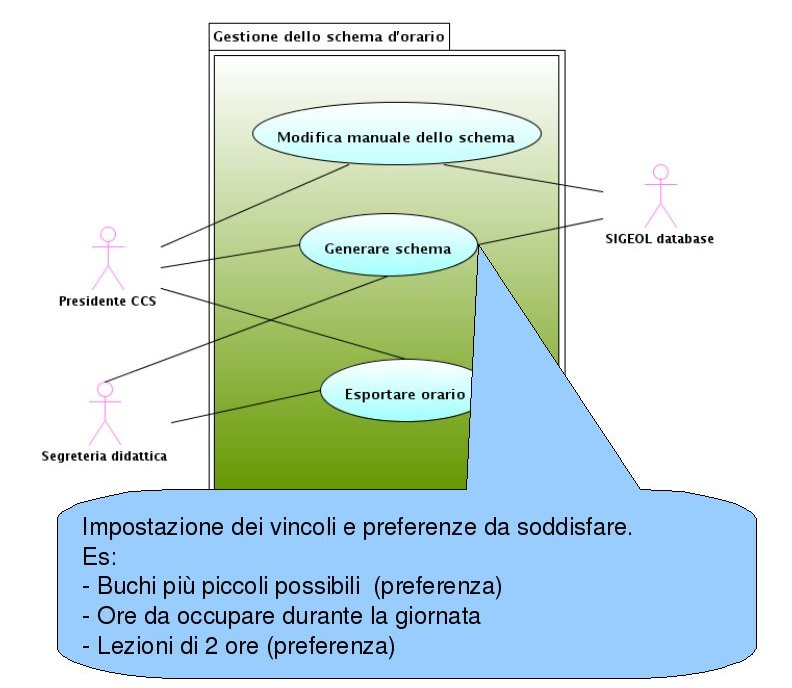
\includegraphics[scale=0.3]{PresentazioneSchemaOrario.jpg}
 % PresentazioneSchemaOrario.jpg: 794x1123 pixel, 72dpi, 28.01x39.62 cm, bb=0 0 794 1123
\end{center}

	\transsplitverticalin
	 }
\end{document}
